\documentclass[10pt,a4paper]{article}
\usepackage[utf8]{inputenc}
\usepackage[italian]{babel}
\usepackage{amsmath}
\usepackage{amsfonts}
\usepackage{amssymb}
\usepackage{graphicx}
\usepackage[left=2cm,right=2cm,top=2cm,bottom=2cm]{geometry}
\newcommand{\rem}[1]{[\emph{#1}]}

\author{Gruppo AC \\ Federico Belliardo, Giulia Franchi, Francesco Mazzoncini}
\title{Esercitazione N.6: Amplificatore operazionale: circuiti lineari}
\begin{document}
\maketitle
\section{Scopo dell'esperienza}

Misurare le caratteristiche di amplificatori invertenti e non invertenti realizzati con un op-amp TL081 in fig.\ref{pin}.
\begin{figure}[!htb]
  \centering
  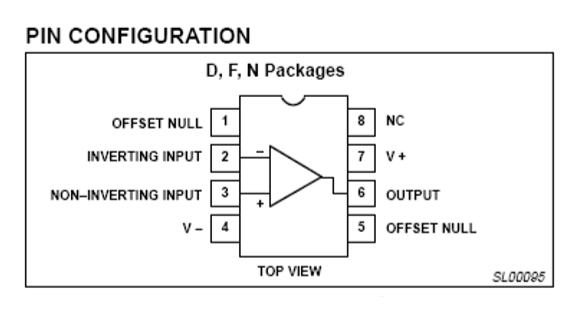
\includegraphics[scale=0.5]{pinrelaz6.png}
\caption{configurazione pin.}
\label{pin}
\end{figure}

\section{Amplificatore invertente}
\subsection{Realizzazione circuito}
Si vuole realizzare un amplificatore invertente con un'impedenza di ingresso superiore a $1k\Omega$ e con un amplificazione di 10. 
Per fare ciò abbiamo montato il circuito in fig. \ref{opampinvert}: Tale circuito infatti presenta una  resistenza di ingresso $R_{in}=R_1$ e un'amplificazione  $A_V=-R_2/R_1$ .\\
Si sono scelte $R_1=2.18 \pm 0.02 \, k\Omega$ e $R_2=21.5 \pm0.02 \, k\Omega$ e abbiamo inoltre misurato le  tensioni di alimentazione dell'OpAmp $V_+=14.99 \pm 0.08 \, V$ $V_-=-15.00 \pm 0.08$.\\
Con questo circuito la resistenza interna attesa è quindi $R_{in.ATT}= R_1 = 2.18 \pm 0.02 \, k\Omega$ e $A_{V.ATT}= -9.9 \pm 0.1$ in accordo con le richieste.\\

\begin{figure}[!htb]
  \centering
  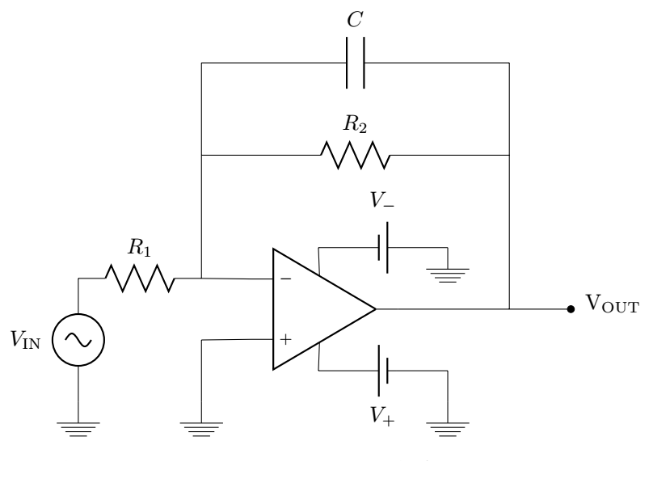
\includegraphics[scale=0.5]{opampinvert.png}
\caption{Schema circuitale amplificatore invertente.}
\label{opampinvert}
\end{figure}

\subsection{Misura del guadagno a frequenza fissata}
Abbiamo misurato per un segnale sinusoidale di frequenza $f=3.00 \pm 0.03 \, kHz$ la tensione picco-picco $V_{OUT}$ in funzione di $V_{IN}$ (sempre picco-picco) riportando i dati nella tabella \ref{tabellaGuadagno}. \\
Abbiamo interrotto la presa dati al valore della tensione in ingresso per il quale abbiamo osservato clipping, misurando però anche il massimo valore della tensione in uscita  $V_{OUT} = 27.0\pm0.2 \, V$ \rem{controllare con il datasheet, perchè non viene trenta.}\\

\begin{table}[!htb]\centering
\begin{tabular}{|c|c|c|c|c|c|}
\hline
$V_{IN} (V)$ & $ \sigma V_{IN} (V)$ & $ V_{OUT} (V)$ & $ \sigma V_{OUT} (V)$ & $A_V$ & $\sigma A_V$\\  
\hline
2.74 & 0.02 & 26.6 & 0.2 & -9.7 & 0.1\\
2.28 & 0.02 & 22.4 & 0.2 & -9.8 & 0.1\\
1.80 & 0.02 & 17.6 & 0.2 & -9.8 & 0.2\\
1.29 & 0.01 & 12.6 & 0.1 & -9.8 & 0.1\\
0.904 & 0.008 & 8.80 & 0.08 & -9.7 & 0.1\\
0.624 & 0.008 & 6.00 & 0.08 & -9.6 & 0.2\\
0.464 & 0.004 & 4.64 & 0.04 & -10.0 & 0.1\\
0.316 & 0.002 & 3.12 & 0.02 & -9.87 & 0.09\\
0.232 & 0.002 & 2.28 & 0.02 & -9.8 & 0.1\\
\hline
\end{tabular}
\caption{Dati delle tensioni $V_{IN}$, $V_{OUT}$ e ampiezze calcolate $A_V$.}
\label{tabellaGuadagno}
\end{table}

Abbiamo eseguito inoltre un grafico di $V_{OUT}$ in funzione di $V_{IN}$ e un fit con una retta riportato in fig. \ref{rettaGuadagno} ricavando come guadagno $A_V=9.74\pm0.04$ \footnote{Nella propagazione degli errori e nel fit si è trascurato l'errore sistematico di calibrazione del  $3\%$ dell'oscilloscopio perchè questo tende a semplificarsi del rapporto di due tensioni.}, compatibile entro l'errore con il guadagno atteso.\\

Per il fit si è utilizzata la funzione \emph{curvefit} della libreria \emph{pylab} con l'opzione \emph{$absolute\,sigma = "true"$}, poichè abbiamo considerando gli errori come statistici. Riportiamo di seguito parametri $m$ e $q$ della retta $y=mx+q$, con la relativa matrice di covarianza: $m = 9.74 \pm 0.04$, $q = 0.03\pm 0.03 \, V$,  $ \Sigma_{ij} = \left( \begin{array}{cc}
2.10 \cdot 10^{-3} & -7.54 \cdot 10^{-4} \\ 
-7.54 \cdot 10^{-4} & 4.37 \cdot 10^{-4}\\
\end{array} \right)$. Con un $\chi^2/ndof = 8.4/7$.\\


\begin{figure}[!htb]
  \centering
  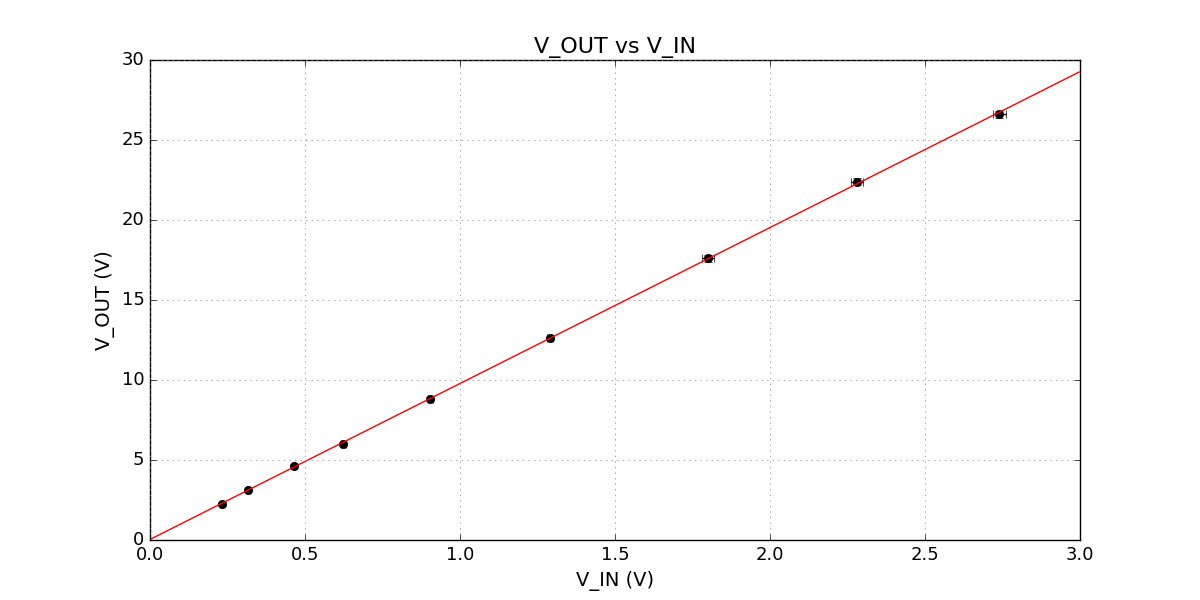
\includegraphics[scale=0.5]{plotGuadagno.png}
\caption{Fit della tensione $V_{OUT}$ in funzione di $V_{IN}$.}
\label{rettaGuadagno}
\end{figure}

\subsection{Misura dell'impedenza d'ingresso}
Abbiamo misurato la tensione di uscita del circuito a $V_{IN}=1.00 \pm 0.01 \, V$, in modo da evitare fenomeni di clipping, dapprima con lo stesso circuito,poi successivamente aggiugendo una resistenza $R_S=2.19 \pm 0.02 \, k \Omega$ \footnote{$R_S$ è stata scelta dello stesso ordine della resistenza interna attesa, in modo da non alterare troppo il circuito, ma più grande, in modo da minimizzare l'incertezza} in serie al generatore di funzioni, ottenendo rispettivamente $V_1=9.68 \pm 0.08 \, V$ e $V_2= 4.88 \pm 0.04 \, V$ Dalla formula del partitore otteniamo $R_S/R_{IN}=\frac{V_1}{V_2}-1$, cioè:
$R_{IN} = R_S \frac{1}{\frac{V_1}{V_2}-1} = 2.22 \pm 0.06 \, k \Omega$, in buon accordo con quella prevista entro l'errore sperimentale.

\section{Risposta in frequenza del circuito e slew rate}
\subsection{Misura della risposta in frequenza}

Abbiamo studiato la risposta in frequenza del circuito misurando $V_{OUT}$ al variare della frequenza (scegliere l'intervallo) con $V_{IN}=0.800 \pm 0.008 \, V$  sinusoidale fissata \footnote{$V_{IN}$ è stata scelta in modo da non avere effetti di distorsione e ci siamo accertati che l'ampiezza del segnale in ingresso rimanesse costante al variare della frequenza, avendo cura in caso di necessità di agire sul generatore di funzioni in modo da avere il segnale voluto.} \\
I dati ottenuto sono stati riportati nella tabella \ref{tabellaBode} e sono stati graficati in un diagramma di Bode in fig. \ref{graficoBode}.\\
Le frequenze sono state misurate con il frequenzimetro dell'oscilloscopio, ad esse si è assegnato un errore dell'$1\%$, poiché è anche l'errore con cui riusciremmo a stimare il periodo con il cursore dei tempi.\\

\begin{table}[!htb]\centering
\begin{tabular}{|c|c|c|c|}
\hline
$f (kHz)$ & $\sigma f (kHz) $ & $ V_{OUT} (V)$ & $\sigma V_{OUT} (V)$\\
\hline
0.00511 & 0.00005 & 7.84 & 0.08\\
0.0098 & 0.0001 & 7.76 & 0.08\\
0.0292 & 0.0003 & 7.76 & 0.08\\
0.102 & 0.001 & 7.92 & 0.08\\
0.307 & 0.003 & 7.92 & 0.08\\
1.02 & 0.01 & 8.00 & 0.08\\
3.04 & 0.03 & 8.00 & 0.08\\
10.2 & 0.1 & 8.00 & 0.08\\
30.9 & 0.3 & 7.84 & 0.08\\
48.2 & 0.5 & 7.52 & 0.04\\
92.7 & 0.9 & 7.04 & 0.04\\
156 & 2 & 6.36 & 0.04\\
212 & 2 & 5.64 & 0.04\\
312 & 3 & 4.36 & 0.02\\
505 & 5 & 2.98 & 0.02\\
704 & 7 & 2.16 & 0.02\\
1000 & 10 & 1.560 & 0.008\\
1600 & 20 & 0.904 & 0.008\\
\hline
\end{tabular}
\caption{Frequenze $f$ del segnale il ingresso e relativo $V_{OUT}$ picco-picco misurato.}
\label{tabellaBode}
\end{table}

Abbiamo notato che il circuito si comporta come un filtro passa-basso ed abbiamo quindi  eseguito un fit con la funzione $ A=\frac{A_{MAX}}{\sqrt{1+(f/f_t)^2}}$.
\rem{vedere se Amax è compatibile con il guadagno massimo dei primi punti}

\begin{figure}[!htb]
  \centering
  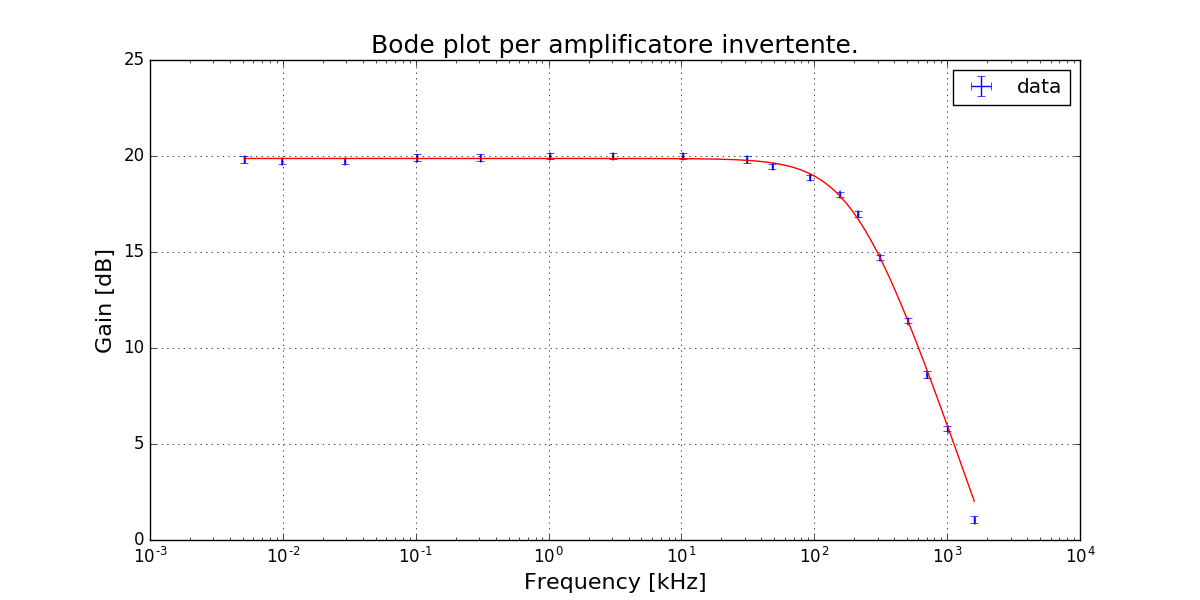
\includegraphics[scale=0.5]{bodePlot.png}
\caption{Plot di Bode amplificatore invertente.}
\label{graficoBode}
\end{figure}

Il fit fornisce: $f_T = 206 \pm 4 \, kHz$ e $A_{max} = 9.85 \pm 0.04$, con matrice di covarianza:
$ \Sigma_{ij} = \left( \begin{array}{cc}
14.1 & -6.23 \cdot 10^{-2} \\ 
-6.23 \cdot 10^{-2} & 1.57 \cdot 10^{-3}\\
\end{array} \right)$. Con un $\chi^2/ndof = 4.46/16$.\\


\subsection{Slew rate}
Abbiamo impostato il generatore di funzioni in modo che fornisse al circuito un’onda quadra. Si è studiato l'andamento di $V_{OUT}$ nella parte del segnale corrispondente al transiente fra i due stati dell’onda: la tensione osservata presenta inizialmente un andamento qualitativamente esponenziale, successivamente un andamento lineare per poi rallentare \rem{?} in prossimità del suo valore limite.\\
Nella zona di crescita lineare si è dunque presa una misura della differenza di tensione $dV_{OUT} = 1.00 \pm 0.02 \, V$ relativa a un piccolo intervallo di tempo $dt=90 \pm 1 \, ns$. Dal loro rapporto si ottiene il valore dello $\emph{slew rate}= 11.1 \pm 0.3 \, \frac{V}{\mu s}$. Il \emph{datasheet} dell'integrato riporta un valore nominale di $13 \frac{V}{\mu s}$ che non è compatibile entro l'errore con il valore misurato, ma un valore di $11 \frac{V}{\mu s}$ rientra nella variabilità del processo di costruzione.

\section{Amplificatore non invertente}
Abbiamo montato il circuito in fig. \ref{opampnoninvert} con $R_1=218 \pm 2 \,  \Omega$ e  un potenziometro di resistenza massima $P_{1_{MAX}}= 97.8 \pm 0.8 \, k\Omega$. La tensione di ingresso è stata fissata a 

\begin{figure}[!htb]
  \centering
  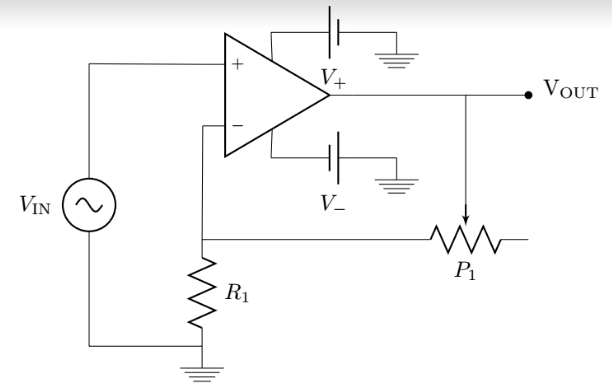
\includegraphics[scale=0.5]{opampnoninvert.png}
\caption{amplificatore non invertente.}
\label{opampnoninvert}
\end{figure}

\begin{table}[!htb]\centering
\begin{tabular}{|c|c|c|c|c|c|c|c|}
\hline
\hline
17.4 & 0.2 & 41.0 & 0.4 & 51.2 & 0.7 & 2100 & 30\\
6.56 & 0.02 & 111 & 1 & 19.3 & 0.1 & 2140 & 10\\
1.96 & 0.02 & 380 & 4 & 5.76 & 0.07 & 2190 & 30\\
4.00 & 0.04 & 187 & 2 & 11.8 & 0.1 & 2200 & 30\\
13.0 & 0.1 & 55.0 & 0.6 & 38.2 & 0.4 & 2100 & 20\\
\hline
\end{tabular}
\caption{Inserire la caption}
\label{Inserire la label}
\end{table}

Abbiamo utilizzato come segnale di ingresso fornito dal generatore di funzioni  un onda sinusoidale di ampiezza $V_{IN}=$\footnote{Anche in questo caso abbiamo eseguito le accortezze sperimentali descritte nella nota precedente.}.\\
\section{Circuito integratore}
\begin{figure}[!htb]
  \centering
  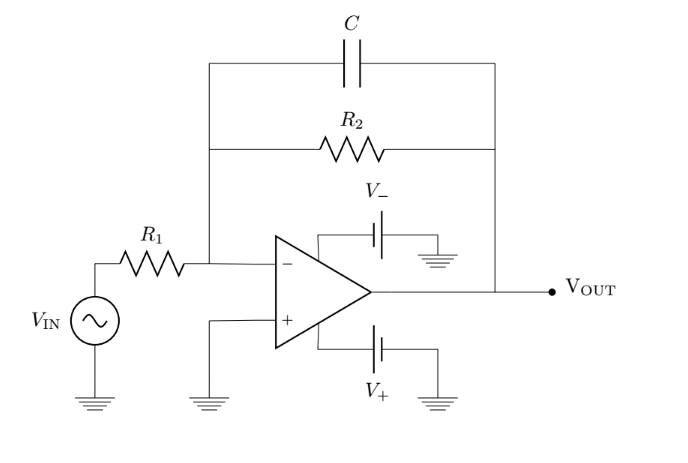
\includegraphics[scale=0.5]{integratore.png}
\caption{circuito integratore con OpAmp}
\end{figure}
\section{Circuito derivatore}
\begin{figure}[!htb]
  \centering
  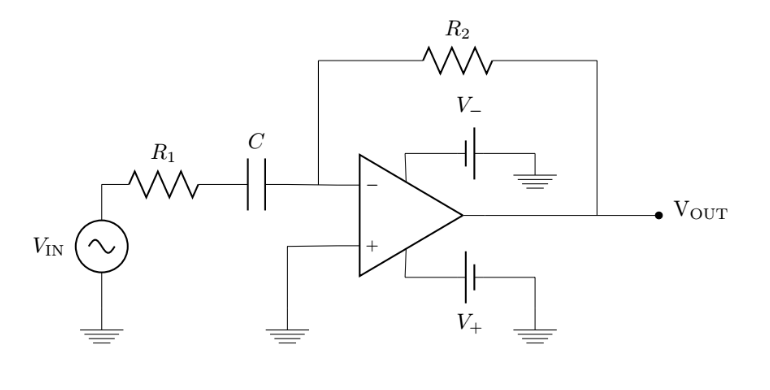
\includegraphics[scale=0.5]{derivatore.png}
\caption{circuito derivatore con OpAmp}
\end{figure}
\end{document}